\section{Solução proposta}

\begin{frame}		
	\begin{block}{Solução proposta}
		A solução proposta neste mestrado recomenda atividades usando três conceitos importantes na área de \emph{workflows} científicos: i) frequência de atividades; ii) compatibilidade entre entrada e saída; e ii) semântica de atividades
	\end{block}
\end{frame}


\begin{frame}		
	\begin{block}{Desenvolvimento da Ontologia}
		A ontologia foi desenvolvida usando a metodologia \emph{Skeletal}, que contém as seguintes fases:
		\begin{enumerate}
			\item Identificar a finalidade;
			\item Construção da ontologia:
			\begin{enumerate}
				\item Captura da ontologia;
				\item Codificação da ontologia;
				\item Integração com ontologias existentes;
			\end{enumerate}
			\item Validação;
			\item Documentação.
		\end{enumerate}
	\end{block}
\end{frame}


\begin{frame}		
	\begin{block}{Matriz para técnicas da literatura}
		\begin{table}[htb]
			\centering
			\caption{Exemplo de matriz de entrada para técnicas da literatura correlata}
			\begin{tabular}{|c|c|c|c|c|}  \hline
				\textbf{\emph{Workflow}} & \textbf{Ativ \(\mathbf{01}\)} & \textbf{Ativ \(\mathbf{02}\)} & \textbf{\(\mathbf{\ldots}\)} & \textbf{Ativ \(\mathbf{280}\)}  \\ \hline
				01 			  & 1 			  & 0 			  & \(\ldots\) 	  & 0  				\\ \hline
				02 			  & 1 			  & 1 			  & \(\ldots\) 	  & 1  				\\ \hline
				03 			  & 1 			  & 0 			  & \(\ldots\) 	  & 1  				\\ \hline
				\(\vdots\) 		  			  & \(\vdots\) 	  & \(\vdots\) 	  & \(\vdots\) 	  & \(\vdots\) 		\\ \hline
				73 			  & 1 			  & 0 			  & \(\ldots\) 	  & 0  				\\ \hline
			\end{tabular}
			\label{tabela_matriz_de_dados}
			%\vspace{0.1cm}
			%\source{\varAutorData}
		\end{table}
	\end{block}
\end{frame}


\begin{frame}		
	\begin{block}{Matriz para técnicas da classificação}
		São usadas as \(59\) atividades mais frequentes, para garantir o balanceamento do classificador estas são replicadas.
		\begin{table}[!htb]
			\tiny
			\centering
			%\caption{Exemplo de matriz de entrada para técnicas de classificação e regressão}
			\begin{tabular}{|c|c|c|c|c|c|c|c|c|}  \hline
				\textbf{\(\#\)} & \textbf{\emph{Workflow}} & \textbf{Ativ \(\mathbf{01}\)} & \textbf{Ativ \(\mathbf{02}\)} & \textbf{\(\mathbf{\ldots}\)}  & \textbf{Ativ \(\mathbf{279}\)} & \textbf{Ativ \(\mathbf{280}\)} & \textbf{Rótulo} \\ \hline
				
				1	&		01		 			   & 1 			  & 0 			  & \(\ldots\) 	  & 0 & 0  			& T	\\ \hline
				2	&		01 					   & 1 			  & 0 			  & \(\ldots\) 	  & 0 & 0  			& T	\\ \hline
				\(\vdots\)  &  \(\vdots\) 	   	   & \(\vdots\)   & \(\vdots\) 	  & \(\vdots\) 	  & \(\vdots\) & \(\vdots\) & \(\vdots\)\\ \hline
				59	&		01 					   & 1 			  & 0 			  & \(\ldots\) 	  & 0 & 0   		& T	\\ \hline
				1	&		01		 			   & 0 (removida) 		  & 1 (adicionada) &\(\ldots\)& 1 & 0	& F	\\ \hline
				2	&		01 					   & 0 (removida)& 0 		  & \(\ldots\) 	  & 1 (adicionada) & 0& F	\\ \hline
				\(\vdots\)  &		\(\vdots\) 	   & \(\vdots\) & \(\vdots\) 	  & \(\vdots\) 	  & \(\vdots\) & \(\vdots\) & \(\vdots\) \\ \hline
				59	&		01 					   & 0 (removida)			  & 0 			  & \(\ldots\) & 0 & 1 (adicionada)& F \\ \hline
				&\(\vdots\) & & & & & & 																		\\ \hline
				1	&		73		 			   & 1 			  & 1  & \(\ldots\) 	  & 0 & 0  			& T	\\ \hline
				2	&		73 					   & 1 			  & 1  & \(\ldots\) 	  & 0 & 0  			& T	\\ \hline
				\(\vdots\)  &		\(\vdots\) 	   & \(\vdots\)   & \(\vdots\) 	  & \(\vdots\) 	  & \(\vdots\) & \(\vdots\) & \(\vdots\) \\ \hline
				59	&		73 					   & 1 			  & 1  & \(\ldots\) 	  & 0 & 0   		& T	\\ \hline
				1	&		73		 			   & 1 (adicionada) & 0 (removida)  & \(\ldots\) 	  & 1 & 0   		& F	\\ \hline
				2	&		73 					   & 1 			  & 0 (removida)  & \(\ldots\)& 1 (adicionada) & 0  & F	\\ \hline
				\(\vdots\)  &		\(\vdots\) 	   & \(\vdots\)   & \(\vdots\) 	  & \(\vdots\) 	  & \(\vdots\) & \(\vdots\) & \(\vdots\)	\\ \hline
				59	&		73 					   & 1 			  & 0 (removida)  & \(\ldots\) 	  & 0 & 1 (adicionada) & F	\\ \hline
			\end{tabular}
			\label{tabela_matriz_de_dados_adapatada_classificacao_regressao}
			%\vspace{0.1cm}
			%\source{\varAutorData}
		\end{table}
	\end{block}
\end{frame}



\begin{frame}		
	\begin{block}{Técnica proposta}
		Para explicar a técnica proposta será usada a figura:
				\begin{figure}
					\begin{minipage}[b]{0.8\textwidth}
						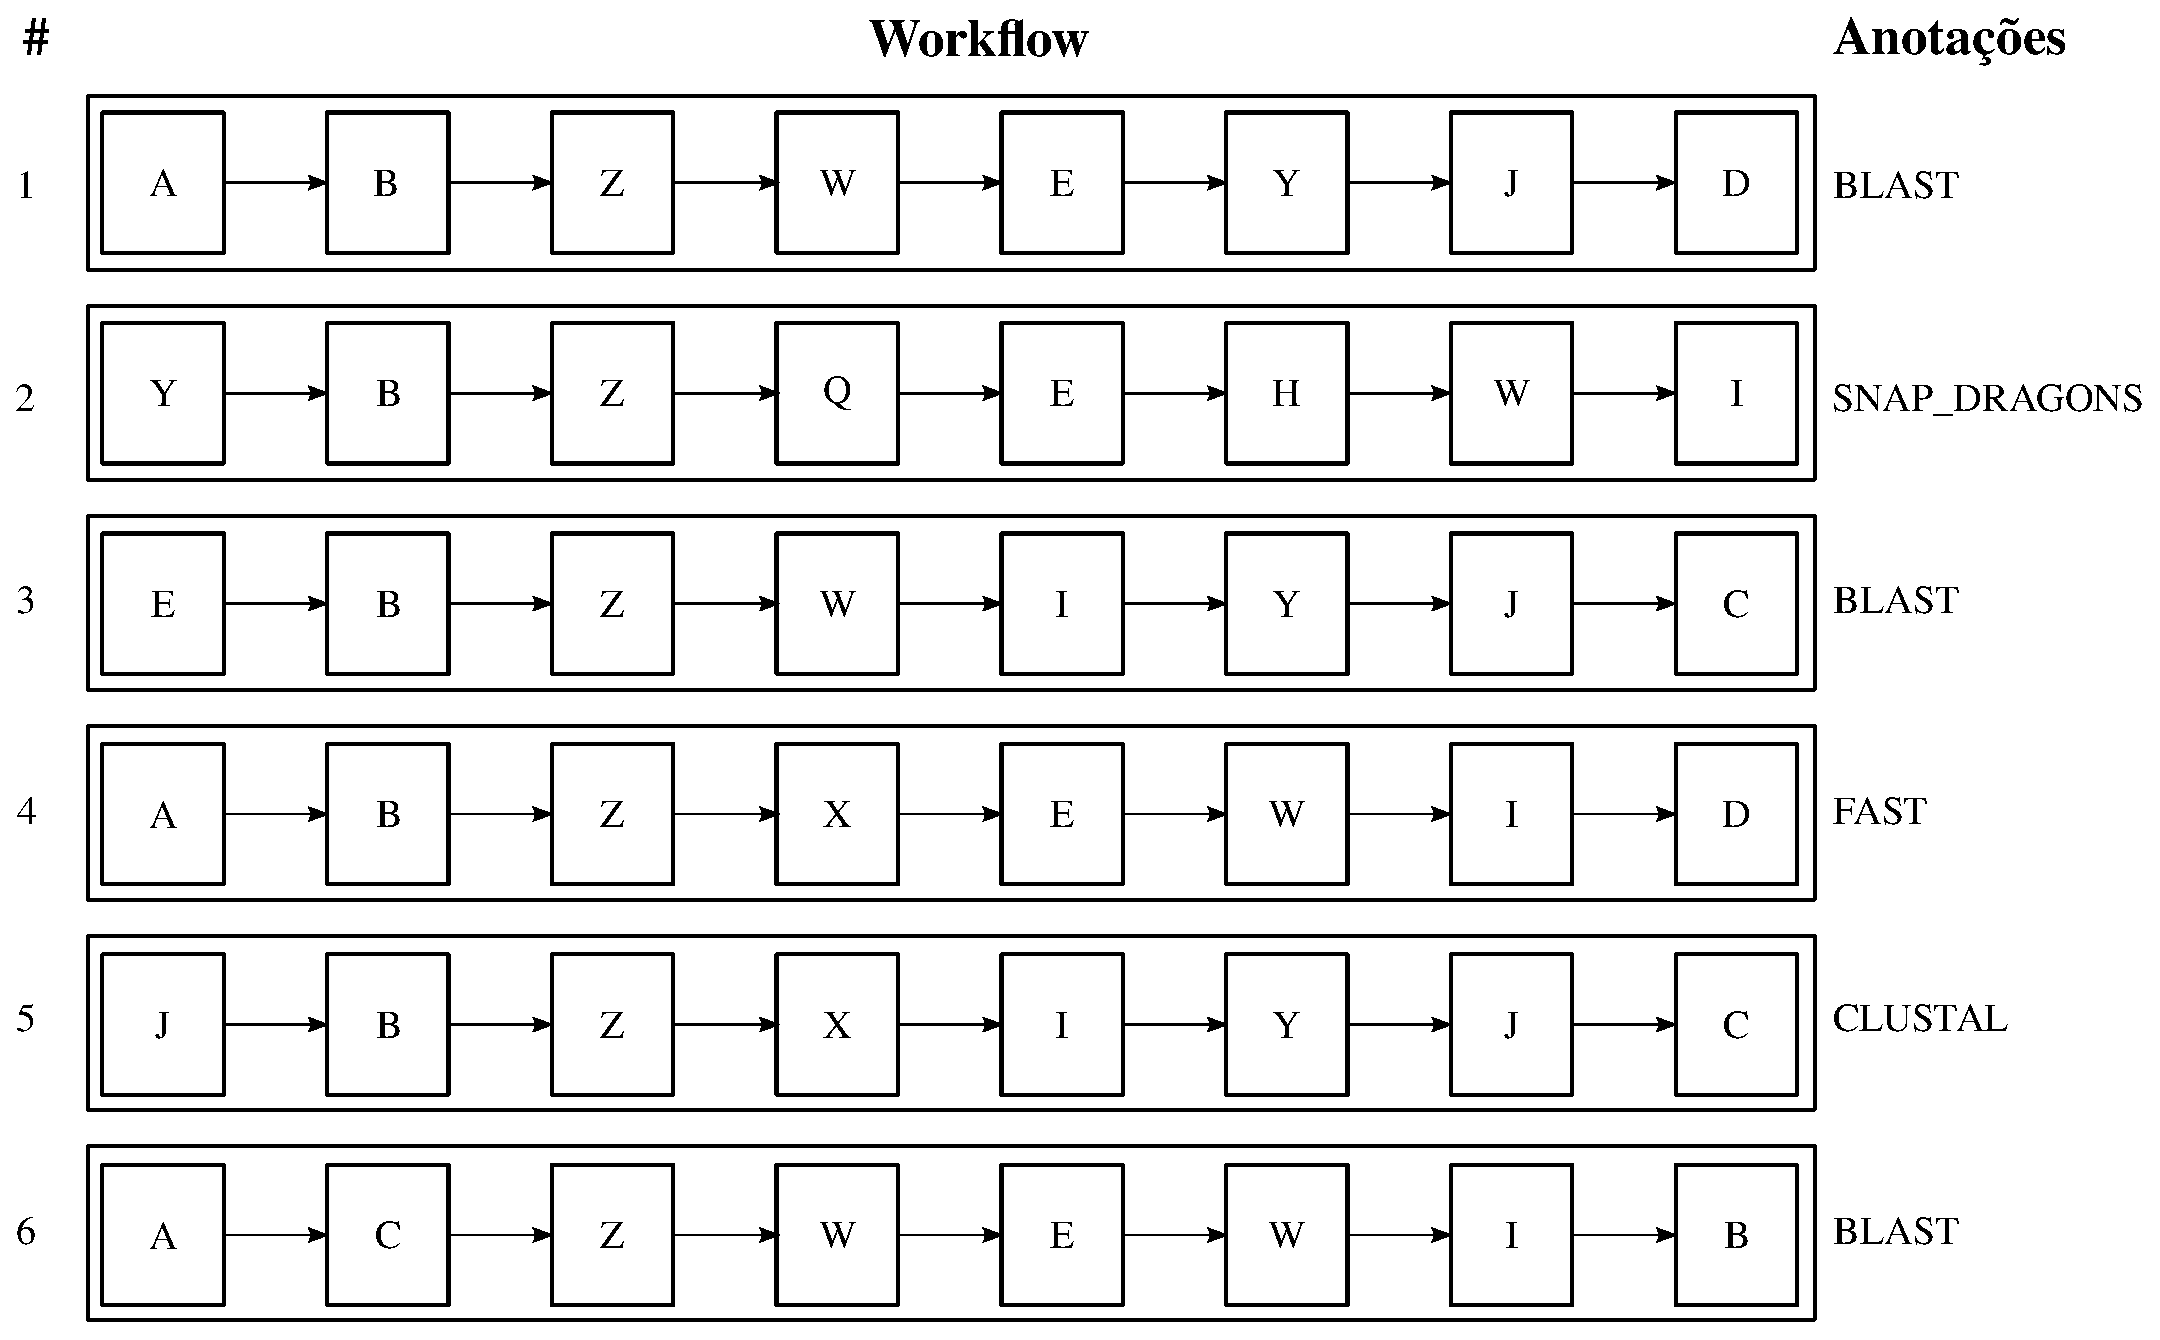
\includegraphics[width=\textwidth]{./secoes/SolucaoProposta/recomendacaofreqontologia.eps}
						\caption{Exemplo de banco de dados de \emph{workflows} científicos}
					\end{minipage}
				\end{figure}
	\end{block}
\end{frame}


\begin{frame}		
	\begin{block}{Técnica proposta}
		Recomendação para a atividade \emph{Z} ordenada por frequência e conceito ontológico.
		\begin{table}[!htb]
			\centering
			%\caption{Recomendação para a atividade \emph{Z} ordenada por frequência e conceito ontológico}
			\begin{tabular}{|c|c|c|c|}  \hline
				\textbf{Posição na Lista} & \textbf{Ativ} & \textbf{Frequência} & \textbf{Anotação Atividade} 	\\ \hline
				1				& W 				& 3 				& BLAST				\\ \hline
				2				& X 				& 2 				& FAST, CLUSTAL		\\ \hline
				3				& Q 				& 1 				& SNAP DRAGONS		\\ \hline
				\(\vdots\)		& \(\vdots\)		& \(\vdots\) 		& \(\vdots\)		\\ \hline
				280				& \(\vdots\)		& \(\vdots\)		& \(\vdots\)	\\ \hline
			\end{tabular}
			\label{tabela_lista_recomendacao_ordenada_frequencia}
			%\vspace{0.1cm}
			%\source{\varAutorData}
		\end{table}		
	\end{block}
\end{frame}